\begin{savequote}[75mm]
%This is some random quote to start off the chapter.
%\qauthor{Firstname lastname}
\end{savequote}

\chapter{Estimation}
{\lettrine[lines=3,slope=1pt,nindent=1pt,]{\textcolor{SchoolColor}{T}}{o estimate the tolerance level in Chicago}, this paper simulates the sorting process through the extended Schelling algorithm and then matches several racial segregation indices to Chicago. Widely used by Urban Economists and Sociologists, the Racial Isolation Index and Racial Dissimilarity Index measure different aspects of segregation. The racial isolation index reflects the probability that a minority person lives nears a majority person or with another minority person. The dissimilarity index measures the percentage of a group's population that would have to change residences for each neighborhood to have the same percentage of that group as the metropolitan area overall. Other potential measures of segregation include the Gini coefficient, entropy, and concentration. However, these measures require data with higher resolution than Census tracts. Racial Isolation (``RII'') and Dissimilarity (``RDI'') are calculated as in Equations \ref{eq:rii} and \ref{eq:rdi}, respectively. For the RDI, the ``other race'' is calculated for race $r$ with ``not-$r$'' as the other race \cite{cutler99}.

The simulated city of Chicago is a 90 $\times$ 42 matrix where 92\% of houses are occuppied with a house price gradient evaluation. This matrix was chosen as it has a similar shape and similar amount of vacant house to Chicago. Additionally, neighborhoods do not overlap when we using the Morse neighborhood concept. As previously stated, agents are defined by race and wealth. With 2.896 million people in 2000 and 2.698 million people in 2010, each agent in the model represents $\sim$700 people. Using a Intel(R) Core(TM) i7-5500U CPU @ 2.40GHz, 2401 Mhz, 2 Core(s), 4 Logical Processor(s) in Rstudio Version 0.99.896, the total time for all simulations (both years) was $\sim$ 14 hours. Most of the time was actually taken up by the $\tau = 40\%$ and  $\tau = 50\%$ simulations, which in total took $\sim$ 8.2 hours, over 50\% of the total computation time. This is because more Schelling steps are required at higher tolerance levels and the number of Schelling steps required grows quickly. For this reason, the simulation was stopped at the first step for which less than 10\% \textit{unsatisfied} agents remained. Without that constraint, the process could have continued for an indefinite period of time. Potentially, this constraint biases the segregation indices downwards because some of the final steps, during which further segregation might occur, are not realized. 

\section{Results}

This paper runs 100 simulations for each tolerance level with each racial and wealth makeup of Chicago. For each simulation, the racial segregation statistics are calculated and stored. The tables below are summary tables for the racial segregation statistics.

\begin{table}[h!]
\centering
\caption[Racial Isolation, 2000 makeup of Chicago]{Racial Isolation Index for varying Tolerance levels in 2000 makeup of Chicago}
\label{RII.2000}
\scalebox{0.85}{
\begin{tabular}{lllllllllllll}
\hline
\multicolumn{13}{l}{Racial Isolation Index for varying Tolerance levels in 2000 makeup of Chicago} \\ \hline \hline
\multicolumn{1}{l|}{}         & \multicolumn{4}{l|}{$\tau = 0\%$}            & \multicolumn{4}{l|}{$\tau = 10\%$}           & \multicolumn{4}{l}{$\tau = 20\%$} \\ \cline{2-13} 
\multicolumn{1}{l|}{}         & Mean & S.D. & Min & \multicolumn{1}{l|}{Max} & Mean & S.D. & Min & \multicolumn{1}{l|}{Max} & Mean    & S.D.    & Min    & Max   \\ \hline
\multicolumn{1}{l|}{White}    & $0.388$ & $0.018$ & $0.329$ & \multicolumn{1}{l|}{$0.433$} & $0.403$ & $0.017$ & $0.366$ & \multicolumn{1}{l|}{$0.451$} & $0.484$ & $0.024$ & $0.434$ & $0.550$\\
\multicolumn{1}{l|}{Black}    & $0.126$ & $0.014$ & $0.092$ & \multicolumn{1}{l|}{$0.172$} & $0.155$ & $0.016$ & $0.116$ & \multicolumn{1}{l|}{$0.198$} & $0.316$ & $0.029$ & $0.257$ & $0.401$\\
\multicolumn{1}{l|}{Hispanic} & $0.062$ & $0.011$ & $0.035$ & \multicolumn{1}{l|}{$0.094$} & $0.091$ & $0.015$ & $0.053$ & \multicolumn{1}{l|}{$0.129$} & $0.194$ & $0.028$ & $0.145$ & $0.254$\\ \hline
\multicolumn{1}{l|}{}         & \multicolumn{4}{l|}{$\tau = 30\%$}           & \multicolumn{4}{l|}{$\tau = 40\%$}           & \multicolumn{4}{l}{$\tau = 50\%$} \\ \cline{2-13} 
\multicolumn{1}{l|}{}         & Mean & S.D. & Min & \multicolumn{1}{l|}{Max} & Mean & S.D. & Min & \multicolumn{1}{l|}{Max} & Mean    & S.D.    & Min    & Max   \\ \hline
\multicolumn{1}{l|}{White}    & $0.609$ & $0.023$ & $0.554$ & \multicolumn{1}{l|}{$0.661$} & $0.729$ & $0.022$ & $0.681$ & \multicolumn{1}{l|}{$0.787$} & $0.829$ & $0.024$ & $0.773$ & $0.881$ \\
\multicolumn{1}{l|}{Black}    & $0.489$ & $0.029$ & $0.402$ & \multicolumn{1}{l|}{$0.559$} & $0.602$ & $0.033$ & $0.508$ & \multicolumn{1}{l|}{$0.718$} & $0.710$ & $0.036$ & $0.629$ & $0.795$ \\
\multicolumn{1}{l|}{Hispanic} & $0.286$ & $0.036$ & $0.205$ & \multicolumn{1}{l|}{$0.377$} & $0.464$ & $0.038$ & $0.388$ & \multicolumn{1}{l|}{$0.554$} & $0.624$ & $0.046$ & $0.504$ & $0.724$ \\ \hline \hline
\end{tabular}
}
\end{table}

Table \ref{RII.2000} presents the RII for the 2000 make of Chicago. One can see that the mean for the index increases monotonically when the tolerance level increases. This means that as individuals have a higher taste for segregation, cities become more segregated. The bounds of the index are quite small, which allows us to make more precise inferences. There is only slight overlapping between the chosen tolerance levels, and the means monotonically increase with tolerance levels. Interestingly, the RII is both lower and varies more for races that are a small fraction of the population. This is a common critique of this measure, but not of the RDI, which is invariant to population size. However, given the sample size and distribution, as well as the tight bounds, these statistics can be accepted with high confidence. We find similar results for for table \ref{RII.2010}.

\begin{table}[h!]
\centering
\caption[Racial Dissimilarity, 2000 makeup of Chicago]{Racial Dissimilarity Index for varying Tolerance levels in 2000 makeup of Chicago}
\label{RDI.2000}
\scalebox{0.85}{
\begin{tabular}{lllllllllllll}
\hline
\multicolumn{13}{l}{Racial Dissimilarity Index for varying Tolerance levels in 2000 makeup of Chicago} \\ \hline \hline
\multicolumn{1}{l|}{}         & \multicolumn{4}{l|}{$\tau = 0\%$}            & \multicolumn{4}{l|}{$\tau = 10\%$}           & \multicolumn{4}{l}{$\tau = 20\%$} \\ \cline{2-13} 
\multicolumn{1}{l|}{}         & Mean & S.D. & Min & \multicolumn{1}{l|}{Max} & Mean & S.D. & Min & \multicolumn{1}{l|}{Max} & Mean    & S.D.    & Min    & Max   \\ \hline
\multicolumn{1}{l|}{White}    & $0.240$ & $0.085$ & $0.156$ & \multicolumn{1}{l|}{$0.371$} & $0.240$ & $0.084$ & $0.158$ & \multicolumn{1}{l|}{$0.397$} & $0.288$ & $0.103$ & $0.197$ & $0.469$ \\
\multicolumn{1}{l|}{Black}    & $0.168$ & $0.044$ & $0.082$ & \multicolumn{1}{l|}{$0.241$} & $0.158$ & $0.042$ & $0.073$ & \multicolumn{1}{l|}{$0.229$} & $0.260$ & $0.071$ & $0.126$ & $0.379$ \\
\multicolumn{1}{l|}{Hispanic} & $0.095$ & $0.025$ & $0.043$ & \multicolumn{1}{l|}{$0.148$} & $0.134$ & $0.033$ & $0.055$ & \multicolumn{1}{l|}{$0.196$} & $0.250$ & $0.042$ & $0.126$ & $0.333$ \\ \hline
\multicolumn{1}{l|}{}         & \multicolumn{4}{l|}{$\tau = 30\%$}           & \multicolumn{4}{l|}{$\tau = 40\%$}           & \multicolumn{4}{l}{$\tau = 50\%$} \\ \cline{2-13} 
\multicolumn{1}{l|}{}         & Mean & S.D. & Min & \multicolumn{1}{l|}{Max} & Mean & S.D. & Min & \multicolumn{1}{l|}{Max} & Mean    & S.D.    & Min    & Max   \\ \hline
\multicolumn{1}{l|}{White}    & $0.387$ & $0.136$ & $0.249$ & \multicolumn{1}{l|}{$0.599$} & $0.592$ & $0.188$ & $0.353$ & \multicolumn{1}{l|}{$0.794$ } & $0.576$ & $0.194$ & $0.352$ & $0.796$ \\
\multicolumn{1}{l|}{Black}    & $0.385$ & $0.107$ & $0.201$ & \multicolumn{1}{l|}{$0.509$} & $0.531$ & $0.167$ & $0.287$ & \multicolumn{1}{l|}{$0.727$}  & $0.515$ & $0.170$ & $0.278$ & $0.727$ \\
\multicolumn{1}{l|}{Hispanic} & $0.327$ & $0.063$ & $0.143$ & \multicolumn{1}{l|}{$0.432$} & $0.556$ & $0.136$ & $0.256$ & \multicolumn{1}{l|}{$0.723$}  & $0.527$ & $0.104$ & $0.240$ & $0.649$ \\ \hline \hline
\end{tabular}
}
\end{table}

In contrast to Table \ref{RII.2000}, Table \ref{RDI.2000} has a much larger standard deviation. The indexes at several tolerance levels overlap each other. However, this reflects the randomness inherent in a Schelling process. As the figures in the Appendix show, there is sometimes large variance in the number of matching agents within a neighborhood. This is especially true for smaller demographics, such as Hispanics or Wealthy agents. Although the means monotonically increase, there is a big jump between 30\% and 40\%. The standard deviations do not increase much with the means, which increases the confidence in the estimated increase in segregation.

\begin{table}[h!]
\centering
\caption[Racial Isolation, 2010 makeup of Chicago]{Racial Isolation Index for varying Tolerance levels in 2010 makeup of Chicago}
\label{RII.2010}
\scalebox{0.85}{
\begin{tabular}{lllllllllllll}
\hline
\multicolumn{13}{l}{Racial Isolation Index for varying Tolerance levels in 2010 makeup of Chicago} \\ \hline \hline
\multicolumn{1}{l|}{}         & \multicolumn{4}{l|}{$\tau = 0\%$}            & \multicolumn{4}{l|}{$\tau = 10\%$}           & \multicolumn{4}{l}{$\tau = 20\%$} \\ \cline{2-13} 
\multicolumn{1}{l|}{}         & Mean & S.D. & Min & \multicolumn{1}{l|}{Max} & Mean & S.D. & Min & \multicolumn{1}{l|}{Max} & Mean    & S.D.    & Min   & Max   \\ \hline
\multicolumn{1}{l|}{White}    & $0.350$ & $0.020$ & $0.310$ & \multicolumn{1}{l|}{$0.401$} & $0.365$ & $0.020$ & $0.300$ & \multicolumn{1}{l|}{$0.402$} & $0.459$ & $0.022$ & $0.394$ & $0.502$ \\
\multicolumn{1}{l|}{Black}    & $0.126$ & $0.014$ & $0.092$ & \multicolumn{1}{l|}{$0.167$} & $0.165$ & $0.018$ & $0.124$ & \multicolumn{1}{l|}{$0.212$} & $0.316$ & $0.027$ & $0.254$ & $0.386$ \\
\multicolumn{1}{l|}{Hispanic} & $0.075$ & $0.012$ & $0.048$ & \multicolumn{1}{l|}{$0.106$} & $0.111$ & $0.017$ & $0.070$ & \multicolumn{1}{l|}{$0.165$} & $0.226$ & $0.026$ & $0.148$ & $0.274$ \\ \hline
\multicolumn{1}{l|}{}         & \multicolumn{4}{l|}{$\tau = 30\%$}           & \multicolumn{4}{l|}{$\tau = 40\%$}           & \multicolumn{4}{l}{$\tau = 50\%$} \\ \cline{2-13} 
\multicolumn{1}{l|}{}         & Mean & S.D. & Min & \multicolumn{1}{l|}{Max} & Mean & S.D. & Min & \multicolumn{1}{l|}{Max} & Mean    & S.D.    & Min    & Max   \\ \hline
\multicolumn{1}{l|}{White}    & $0.599$ & $0.024$ & $0.518$ & \multicolumn{1}{l|}{$0.651$} & $0.729$ & $0.023$ & $0.662$ & \multicolumn{1}{l|}{$0.782$} & $0.830$ & $0.022$ & $0.782$ & $0.895$ \\
\multicolumn{1}{l|}{Black}    & $0.482$ & $0.029$ & $0.403$ & \multicolumn{1}{l|}{$0.556$} & $0.599$ & $0.033$ & $0.531$ & \multicolumn{1}{l|}{$0.680$} & $0.715$ & $0.035$ & $0.632$ & $0.811$ \\
\multicolumn{1}{l|}{Hispanic} & $0.346$ & $0.036$ & $0.263$ & \multicolumn{1}{l|}{$0.428$} & $0.474$ & $0.042$ & $0.365$ & \multicolumn{1}{l|}{$0.584$} & $0.612$ & $0.049$ & $0.471$ & $0.714$ \\ \hline \hline
\end{tabular}
}
\end{table}
\begin{table}[h!]
\centering
\caption[Racial Dissimilarity, 2010 makeup of Chicago]{Racial Dissimilarity Index for varying Tolerance levels in 2010 makeup of Chicago}
\label{RDI.2010}
\scalebox{0.85}{
\begin{tabular}{lllllllllllll}
\hline
\multicolumn{13}{l}{Racial Isolation Index for varying Tolerance levels in 2010 makeup of Chicago} \\ \hline \hline
\multicolumn{1}{l|}{}         & \multicolumn{4}{l|}{$\tau = 0\%$}            & \multicolumn{4}{l|}{$\tau = 10\%$}           & \multicolumn{4}{l}{$\tau = 20\%$} \\ \cline{2-13} 
\multicolumn{1}{l|}{}         & Mean & S.D. & Min & \multicolumn{1}{l|}{Max} & Mean & S.D. & Min & \multicolumn{1}{l|}{Max} & Mean    & S.D.    & Min    & Max   \\ \hline
\multicolumn{1}{l|}{White}    & $0.232$ & $0.079$ & $0.141$ & \multicolumn{1}{l|}{$0.349$} & $0.227$ & $0.080$ & $0.142$ & \multicolumn{1}{l|}{$0.356$} & $0.319$ & $0.104$ & $0.184$ & $0.455$ \\
\multicolumn{1}{l|}{Black}    & $0.151$ & $0.040$ & $0.073$ & \multicolumn{1}{l|}{$0.219$} & $0.151$ & $0.042$ & $0.071$ & \multicolumn{1}{l|}{$0.215$} & $0.248$ & $0.074$ & $0.131$ & $0.358$ \\
\multicolumn{1}{l|}{Hispanic} & $0.099$ & $0.027$ & $0.044$ & \multicolumn{1}{l|}{$0.154$} & $0.142$ & $0.034$ & $0.055$ & \multicolumn{1}{l|}{$0.221$} & $0.254$ & $0.064$ & $0.101$ & $0.337$ \\ \hline
\multicolumn{1}{l|}{}         & \multicolumn{4}{l|}{$\tau = 30\%$}           & \multicolumn{4}{l|}{$\tau = 40\%$}           & \multicolumn{4}{l}{$\tau = 50\%$} \\ \cline{2-13} 
\multicolumn{1}{l|}{}         & Mean & S.D. & Min & \multicolumn{1}{l|}{Max} & Mean & S.D. & Min & \multicolumn{1}{l|}{Max} & Mean    & S.D.    & Min    & Max   \\ \hline
\multicolumn{1}{l|}{White}    & $0.413$ & $0.139$ & $0.237$ & \multicolumn{1}{l|}{$0.599$} & $0.521$ & $0.164$ & $0.312$ & \multicolumn{1}{l|}{$0.711$} & $0.614$ & $0.183$ & $0.353$ & $0.808$ \\
\multicolumn{1}{l|}{Black}    & $0.365$ & $0.108$ & $0.199$ & \multicolumn{1}{l|}{$0.519$} & $0.460$ & $0.135$ & $0.238$ & \multicolumn{1}{l|}{$0.652$} & $0.499$ & $0.172$ & $0.282$ & $0.748$ \\
\multicolumn{1}{l|}{Hispanic} & $0.370$ & $0.075$ & $0.163$ & \multicolumn{1}{l|}{$0.474$} & $0.443$ & $0.113$ & $0.218$ & \multicolumn{1}{l|}{$0.603$} & $0.562$ & $0.124$ & $0.252$ & $0.711$ \\ \hline \hline
\end{tabular}
}
\end{table}

Racial Dissimilarity and Racial Isolation in the following tables both similarly match Chicago's actual 2000 and 2010 values. However, the RII values increase more slowly in tolerance than the RDI values, and the standard deviation of RII is larger. This reflects the differing interpretations of RDI versus RII. RDI is a citywide estimate of the segregation of one race from all other mutually exclusive racial groups, while the RII is a citywide estimate of the segregation of one racial group generally within neighborhoods. The RDI is roughly a measure of how strongly two races clump themselves into largely segregated neighborhoods; this tends to happen quickly, and numerically it is easier for a neighborhood to be largely of one race. The RII, however, is more sensitive to the distribution of one race within a neighborhood, which is more likely to vary because it is more subject to initial conditions. This reflects a peculiarity of the Schelling process; unlike a regular Schelling process, there is not random placement in the city but rather some wealth concentration. Hence, although the wealth inequality drives broader trends in inequality, therefore universally pushing up the RDI, there is still significant random variation within some neighborhoods because, for example, poor Blacks cannot escape into rich White neighborhoods, even if both groups would tolerate that move.

\begin{figure}[!h]
\centering
\begin{subfigure}[b]{.5\textwidth}
  \centering
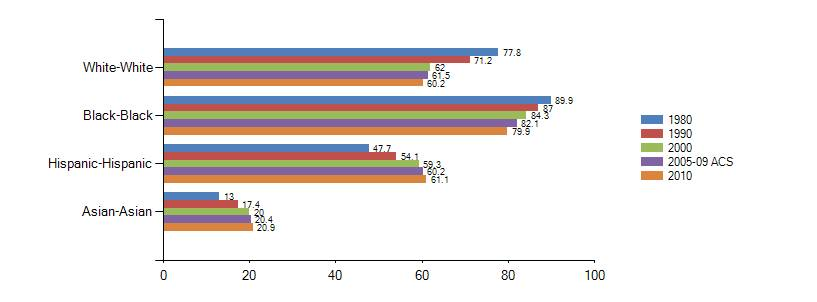
\includegraphics[scale=.35]{figures/chart1.png}
\caption{Racial Dissimilarity Index}
\end{subfigure}%
\begin{subfigure}[b]{.5\textwidth}
  \centering
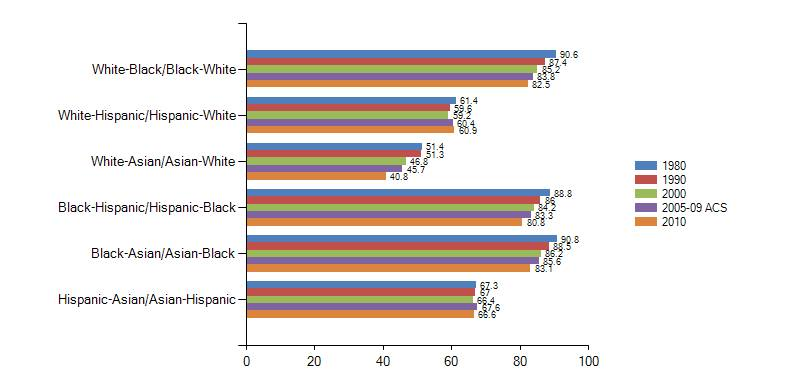
\includegraphics[scale=.35]{figures/chart2.png}
\caption{Racial Isolation Index}
\end{subfigure}
\caption{Actual Segregation Indices for Chicago}
\end{figure}

For both 2000 and 2010 demographics, a 50\% tolerance level is the minimum tolerance level sufficient to reproduce Chicago's segregation statistics on average. Because a 50\% tolerance level is the minimum tolerance level for both parameterizations, we can conclude that if housing choices are made with a Schelling process, Chicago has not become more tolerant in the past decade. Interestingly, 50\% is the amount of housing discrimination the General Social Survey finds that Whites are willing to tolerate, suggesting that there is no ``housing Bradley effect.''\footnote{The Bradley Effect is named for the 1982 California gubernatorial election, in which there was significant response bias to public polling. Bradley, the longtime Los Angeles mayor, lost the election despite leading in the polls. Several have speculated that respondents, despite opposing Bradley, did not want to appear racist in front of pollsters by opposing an ``historic'' election. Therefore, the Bradley Effect has particular racial significance in the context of American politics and public policy beyond polling response bias.} This means that even if Whites are honest about their racial preferences, these relatively benign preferences can result in highly segregated cities, even if the initial conditions are random. In real life, of course, the initial conditions are not randomly distributed; in fact, Chicago is already a highly segregated city, so it is possible that these simulations underestimate how racially tolerant Whites are because the initial conditions are not random. However, Zhang does provide some evidence of invariance to initial conditions in simulation convergence; his proof, however, is not mathematical. In short, more testing and analysis are required.

